% !TEX root = machine_learning.tex





\chapter{Data Visualization and Manifold Learning}
\label{chap:manifold.learning}



\section{Multidimensional scaling}
The methods described in this chapter aim at representing a dataset in low dimension, allowing for its visual exploration by summarizing its structure in a user-accessible interface. Unlike factor analysis methods, they do not necessarily attempt at providing a causal model expressing the data as a function of a small number of sources, and generally do not provide a direct mechanism for adding new data to the representation. 
In addition, all these methods take as input similarity dissimilarity matrices between data points and do not require, say, Euclidean coordinates.

Assuming that a dissimilarity matrix $D = (d_{kl}, \,k,l=1, \ldots, N)$ is given, the goals of multidimensional scaling (or MDS) is to determine a small-dimensional Euclidean representation, say $y_1, \ldots, y_N\in \mR^p$, such that $\abs{y_k - y_l}^2  \simeq
d_{kl}^2$. We review below two versions of this algorithm, referred to as ``similarity'' and ``dissimilarity'' matching.

\subsection{Similarity matching (Euclidean case)}
We start with the standard hypotheses of  MDS, assuming that the distances $d_{kl}$ derive from a representation in feature space, so that $d_{kl}^2 = \|h_k - h_l\|_H^2$ for some inner-product space $H$ and (possibly unknown) features $h_1, \ldots, h_N$. Note that, since the Euclidean distance is invariant by translation, there is no loss of generality in assuming $h_1 + \cdots + h_N=0$, which will be done in the following.

We look for a $p$-dimensional representation in the form  $y_k = \Phi h_k$ where $\Phi$ is a linear transformation (and we want $y_k$ to be computable directly from dissimilarities, since we do not assume that $h_k$ is known). Since we are only interested in a transformation of the $h_1, \ldots, h_N$, it suffices to compute $\Phi$ in the vector space generated by them, so that we let
\[
\Phi: \mathrm{span}(h_1, \ldots, h_N) \to \mR^p\,,
\]
and we want $\Phi$ to
(approximately) conserve the norm, i.e., be close to being an isometry. 

Because isometries are one-to-one and onto, the existence of an exact isometry would require $V \defeq \mathrm{span}(h_1, \ldots, h_N)$ to be $p$-dimensional. The mapping $\Phi$ could then  be defined as $\Phi(h) = (\scp{h}{e_1}_H, \ldots, \scp{h}{e_p}_H)$ where $e_1, \ldots, e_p$ is any orthonormal basis of $V$. In the general case, however, where $V$ is not $p$-dimensional or less, one can  replace it by a best $p$-dimensional approximation of the training data, leading to a problem similar to PCA in feature space.

Indeed, as we have seen in  \cref{sec:pca.comp}, this best approximation can be obtained by diagonalizing the Gram matrix $S$ of $h_1, \ldots, h_N$, which is such that  $s_{kl} = \scp{h_k}{h_l}_H$. (Recall that we assume that $\bar h = 0$, so we do not center the data here.) Using the notation in \cref{sec:pca.comp}, let $\pe \al 1, \ldots, \pe \al p$ denote the eigenvectors associated with the $p$ largest eigenvalues, normalized so that $(\pe \al i)^TS\pe \al i = 1$ for $i=1, \ldots, p$. One can then take
\[
e_i = \sum_{l=1}^N \pe{\al_{l}}i h_l
\]
and, for $k=1, \ldots, N$, $j=1, \ldots, p$:
\begin{equation}
\label{eq:mds.sol}
\pe {y_{k}} i = \la_i^2 \pe{\al_{k}} i
\end{equation}
where $\la_i^2$ is the eigenvalue associated with $\pe \al i$.

This does not entirely address the original problem, since the inner products $s_{kl}$ are not given, but only the  distances $d_{kl}$, which satisfy
\begin{equation}
\label{eq:s.to.d}
 d_{kl }^2 = - 2 s_{kl} + s_{kk} +s_{ll}\,.
\end{equation}
This provides a linear system of equations in the unknown $s_{kl}$.  
This system is under-determined, because  $D$ is invariant by any transformation $h_k \mapsto h_k + h_0$ (for a fixed $h_0$), and $S$ is not. However, the assumption $h_1+\cdots+h_N=0$ provides the additional constraint needed to provide a unique solution. 

Summing  \cref{eq:s.to.d} over $l$, we then get 
\begin{equation}
\label{eq:s.to.d.2}
\sum_{l=1}^N d_{kl}^2 = Ns_{kk} + \sum_{l=1}^N s_{ll}\,.
\end{equation}
Summing this equation over $k$, we find 
\[
\sum_{k,l=1}^N d_{kl}^2 = 2N \sum_{l=1}^N s_{ll}.
\]
Using this in \cref{eq:s.to.d.2}, we get 
\[
s_{kk} = \frac1N\sum_{l=1}^N d_{kl}^2 - \frac1{2N^2} \sum_{k,l=1}^N d_{kl}^2,
\]
and, from \cref{eq:s.to.d}
\[
s_{kl} = -\frac12\left(d_{kl}^2 - \frac1N\sum_{k'=1}^N d_{k'l}^2 - \frac1N\sum_{l'=1}^N d_{kl'}^2 + \frac1{N^2} \sum_{k',l'=1}^N d_{k'l'}^2\right).
\]
If we denote by $D^{\odot 2}$ the matrix formed with the squared distances $d^2_{kl}$, this identity can we rewritten in the simpler form  
\begin{equation}
\label{eq:dissim.sim}
S = -\frac12 P D^{\odot 2} P
\end{equation}
with $P = \Id[N] -\dsone_N \dsone_N^T/N$.


We now show that this PCA approach to MDS is equivalent to the problem of minimizing
\begin{equation}
\label{eq:sim.match}
F(y) = \sum_{k,l=1}^N (y_k^Ty_l - s_{kl})^2 
\end{equation}
over all $y_1, \ldots, y_N\in \mR^p$ such that $y_1 + \cdots + y_N = 0$, 
which can be interpreted as matching ``similarities'' $s_{kl}$ rather than distances. Indeed, letting $\CY$ denote the $N$ by $p$ matrix with rows $y_1^T, \ldots, y_N^T$, we have
\[
F(y) = \trace( (\CY\CY^T - S)^2).
\]
Finding $\CY$ is equivalent to finding a symmetric matrix $M$ of rank $p$ minimizing $\trace((M-S)^2)$.
 We have, using the trace inequality (\cref{th:trace.ineq}), and letting $\la_1^2 \geq \cdots \geq \la_N^2$  (resp. $\mu_1^2 \geq \cdots \geq \mu_p^2$) denote the eigenvalues of $S$ (resp. $M$)
\begin{align*}
\trace((M-S)^2) & = \trace(M^2) - 2\trace(MS) + \trace(S^2) \\
&= \sum_{k=1}^p \mu_k^4 - 2\trace(MS) + \sum_{k=1}^N \la_k^4\\
&\geq \sum_{k=1}^p \mu_k^4 - 2\sum_{k=1}^p \la^2_k\mu^2_k + \sum_{k=1}^N \la_k^2\\
&= \sum_{k=1}^p (\la^2_k-\mu^2_k)^2 + \sum_{k=p+1}^N \la_k^4\\
&\geq  \sum_{k=p+1}^N \la_k^4
\end{align*}
This lower bound is attained when $M$ and $S$ can be diagonalized in the same orthonormal basis with $\la^2_k=\mu^2_k$ for $k=1, \ldots, p$. So, letting $S = UDU^T$, where $U$ is orthogonal and $D$ is diagonal with decreasing numbers on the diagonal, an optimal $M$ is given by $M = U_p D_p U_p^T$, where $U_p$ is formed with the first $p$ columns of $A$ and $D_p$ is the first $p\times p$ block of $D$. This shows that the matrix $\CY = U_p D^{1/2}$ provides a minimizer of $F$.
The matrix $U = [\pe u 1, \ldots, \pe u N]$ differs from the matrix $A = [\pe \al 1, \ldots, \pe \al N]$ above through the normalization of its column vectors: we have $S\pe \al i = \la^2_i \pe \al i$ with $(\pe \al i)^T S \pe \al i = 1$ while $S\pe u i = \la^2_i \pe u i$ with $(\pe u i)^T S \pe u i = \la^2_i$ showing that $\pe \al i = \la_i^{-1} \pe u i$. This shows that $A_p = U_p D_p^{-1/2}$ so that $\CY$ can also be rewritten as $\CY = A_p D_p$, i.e., $\pe {y_{k}} i =  \la_i^2 \pe {\al_{k}} i$, the same expression that was obtained before.

The minimization of $F$ is called {\em similarity matching}. Clearly, this method can be applied when one starts directly with a matrix of dissimilarities $S$, provided it satisfies $\sum_{l=1}^N s_{kl}=0$ for all $k$. If this is not the case, then interpreting $s_{kl}$ as an inner product $h_k^Th_l$, it is natural to replace $s_{kl}$ by what would give $(h_k - \bar h)^T(h_l - \bar h)$, namely, by 
\[
s'_{kl} = s_{kl} - \frac1N \sum_{l'=1}^N s_{kl'} - \frac1N \sum_{ k'=1}^N s_{k' l} + \frac1{N^2} \sum_{k', l'=1}^N s_{k'l'}.
\]  
Interestingly, this discussion provides us with yet another interpretation of PCA.

\subsection{Dissimilarity matching}
While the minimization of \cref{eq:sim.match} did not provide us with a new way of analyzing the data (since it was equivalent to PCA), the direct comparison of dissimilarities, that is, the minimization of 
\[
G(y) = \sum_{k,l=1}^N (|y_k-y_l| - d_{kl})^2
\]
over $y_1, \ldots, y_N\in \mR^p$, provides a different approach.  Since this may be useful in practice and does not bring in much additional difficulty, we will allow for the possibility of weighting the differences in $G$ and consider the minimization of 
\[
G(y) = \sum_{k,l=1}^N w_{kl}(|y_k-y_l| - d_{kl})^2
\]
where $W = (w_{kl})$ is a symmetric matrix of non-negative weights. The only additional complexity resulting by adding weights is that the indeterminacy on $y_1, \ldots, y_N$ is that $G(y)=G(y')$ as soon as $y-y'$ is constant on every connected component of the graph associated with the weight matrix $W$, so that the constraint on $y$ should be replaced by
\[
\sum_{k\in \Ga} y_k = 0
\]
for any connected component $\Ga$ of this graph. (If all weights are positive, then the only non-empty connected component is $\{1, \ldots, N\}$ and we retrieve our previous constraint  $\sum_{k=1}^N y_k = 0$.)

Standard nonlinear optimization methods, such as projected gradient descent, may be used to minimize $G$, but the preferred algorithm for MDS uses a stepwise procedure resulting from the addition of an auxiliary variable.
Rewrite
\[
G(y) = \sum_{k,l=1}^N w_{kl} |y_k-y_l|^2 - 2 \sum_{k,l=1}^N w_{kl} d_{kl} |y_k-y_l| + \sum_{k,l=1}^N d_{kl}^2\,.
\]
We have,  for $u\in \mR^p$: 
\[
|u| = \max\{z^T u: z\in \mR^p, |z| = \bfone_{u\neq 0}\}\,.
\]
Using this identity, we can  introduce auxiliary variables $z_{kl}$, $k,l=1, \ldots, N$ in $\mR^p$, with $|z_{kl}| = 1$ if $y_k\neq y_l$ and  define
\[
\hat G(y,z) = \sum_{k,l=1}^N w_{kl} |y_k-y_l|^2 - 2 \sum_{k,l=1}^N w_{kl} d_{kl} (y_k-y_l)^T z_{kl} + \sum_{k,l=1}^N d_{kl}^2\,.
\]
We then have
\[
G(y) = \min_{z: |z_{kl}|=1 \text{ if } y_k\neq y_k} \hat G(y,z).
\]
As a consequence,  minimizing $G$ in $y$ can be achieved by minimizing $\hat G$ in $y$ and $z$ and discarding $z$ when this is done. One can minimize $\hat G$ iteratively, alternating minimization in $y$ given $z$ and in $z$ given $y$, both steps being elementary. In order to describe these steps, introduce some matrix notation. 

Let $L$ denote the Laplacian matrix of the weighted graph on $\{1, \ldots, N\}$ associated with the weight matrix $W$, namely $L = (\ell_{kl}, k,l=1, \ldots, N)$ with $\ell_{kk} = \sum_{k=1}^N w_{kl} - w_{kk}$ and $\ell_{kl} = -w_{kl}$ when $k\neq l$. Then, 
\[
\sum_{k,l=1}^N w_{kl} |y_k-y_l|^2 = 2 \trace( \CY^T L \CY).
\]
Defining $u_k\in \mR^p$ by
\[
u_k = \sum_{l=1}^N w_{kl} d_{kl} (z_{kl}-z_{lk}),
\]
and $\CU = \begin{pmatrix} u_1^T\\ \vdots \\ u_N^T\end{pmatrix}$, we have
\[
\sum_{k,l=1}^N w_{kl} d_{kl} (y_k-y_l)^T z_{kl} = \trace (\CU^T \CY).
\]
With this notation, the optimal matrix $\CY$ must minimize
\[
2 \trace( \CY^T L \CY) - 2 \trace(\CU^T \CY). 
\]

Let $m$ be the number of connected components of the weighted graph.
Recall that the matrix $L$ is positive semi-definite and that an orthonormal basis of its null space is provided by vectors, say $e_1, \ldots, e_m$, that are constant on each of the $m$ connected components of the graph, so that the constraint on $\CY$ can be written as $e_j^T\CY = 0$ for $j=1, \ldots, m$. Introduce the matrix
\[
\hat L = L + \sum_{k=1}^m e_ke_k^T
\]
which is positive definite. Our minimization problem is then equivalent to minimizing
\[
2 \trace( \CY^T \hat L \CY) - 2 \trace(\CU^T \CY), 
\]
subject to $e_j^T\CY = 0$ for $j=1, \ldots, m$. The derivative of this function is 
\[
 4 \hat L\CY - 2 \CU
\]
so that an optimal $\CY$ must satisfy
\[
4 \hat L\CY - 2 \CU + \sum_{j=1}^m  e_j\mu_j^T = 0
\]
for Lagrange multipliers $\mu_1, \ldots, \mu_m\in \mR^p$. This shows that
\[
\CY = \frac12 \hat L^{-1} \Big(\CU - \frac12 \sum_{j=1}^m  e_j\mu_j^T\Big) =  \frac12 \hat L^{-1} \CU - \frac14 \sum_{j=1}^m  e_j\mu_j^T
\]
where we have used the fact that $\hat L^{-1} e_j = e_j$. We can now identify $\mu_j$ since
\[
0 = e_j^T\CY = \frac12 e_j^T \hat L^{-1} \CU - \frac14 \sum_{j'=1}^m e_j^T e_{j'} \mu_j^T = \frac12 e_j^T \CU - \frac14 \mu_j^T
\]
so that $\mu_j^T = 2 e_j^T\CU$ and the optimal $\CY$ is
\[
\CY = \frac12 \hat L^{-1} \CU - \frac12 \sum_{j=1}^m e_j e_j^T \CU.
\]
Note that this expression can be rewritten as
\[
\CY = \frac12  P_L \hat L^{-1} \CU
\]
where $P_L = \Id[N]  - \sum_{k=1}^N e_je_j^T$ is the projection onto the space perpendicular to the null space of $L$ (i.e., the range of $L$).
In the case where the graph has a single connected component, one has  $m=1$ and $e_1 = \dsone_N/\sqrt N$ yielding
\[
P_L = \Id[N] - \frac1N \dsone_N\dsone_N^T.
\]

The minimization in $z$ given $y$ is straightforward: if $y_k\neq y_k$, then $z_{kl} = (y_k-y_l)/|y_k-y_l|$. If $y_k=y_l$, then one can take any value for $z_{kl}$ and the simplest if of course $z_{kl}=0$. Using the previous computation, we can summarize a training algorithm for multi-dimensional scaling, called SMACOF for ``Scaling by Maximizing a Convex Function'' (see, e.g., \citet{borg2005modern} for more details and references).

\begin{algorithm}[SMACOF]
Assume that a symmetric matrix of dissimilarities $(d_{kl}, k,l=1, \ldots, N)$ is given, together with a matrix of weights $(w_{kl}, k,l=1, \ldots, N)$. Fix a target dimension, $p$. Fix a tolerance constant $\ep$.
\begin{enumerate}[label=\arabic*., wide=0.5cm]
\item Compute the Laplacian matrix $L$ of the graph associated with the weights, the projection matrix $P_L$ onto the range of $L$ and the matrix $M = (L + \Id[N] - P_L)^{-1}$.
\item Initialize the algorithm with some family $y_1, \ldots, y_N \in \mR^p$ and let $\CY = \begin{pmatrix} y_1^T\\ \vdots \\ y_N^T\end{pmatrix}$.
\item At a given step of the algorithm, let $\CY$ be the current solution and compute, for $k=1, \ldots, N$:
\[
u_{k} = 2 \sum_{l=1}^N w_{kl} d_{kl} \frac{y_{k}-y_{l}}{|y_k-y_l|} \bfone_{y_k\neq y_l}
\]
to form the matrix $\CU = \begin{pmatrix} u_1^T\\ \vdots \\ u_N^T\end{pmatrix}$.
\item Compute $\CY' = \frac12  P_L M \CU$.
\item If $|\CY -\CY'| \leq \ep$, exit and return $\CY'$.
\item Return to step 3.
\end{enumerate}
\end{algorithm}


\section{Manifold learning}

The goal of MDS is to map a full matrix of distances into a low-dimensional Euclidean space. Such a representation, however, cannot address the possibility that the data is supported by a low-dimensional, albeit nonlinear, space.  For example, people leaving on Earth live, for all purposes, on a two-dimensional structure (a sphere), but any faithful Euclidean representation of the world population needs to use the three spatial dimensions. One may also argue that the relevant distance between points on Earth is not the Euclidean one either (because one would never travel {\em through}  Earth to go from one place to another), but the distance associated to the shortest path on the sphere, which is measured along great circles.

To take another example, the left panel in \cref{fig:isomap.curve} provides the result of applying MDS to a ten-dimensional dataset obtained by applying a random ten-dimensional rotation to a curve supported by a three-dimensional torus. MDS indeed retrieves the correct curve structure in space, which is  three dimensional. However, for a person ``living'' on the curve, the data is one-dimensional, a fact that is captured by the Isomap method that we now describe.


\begin{figure}
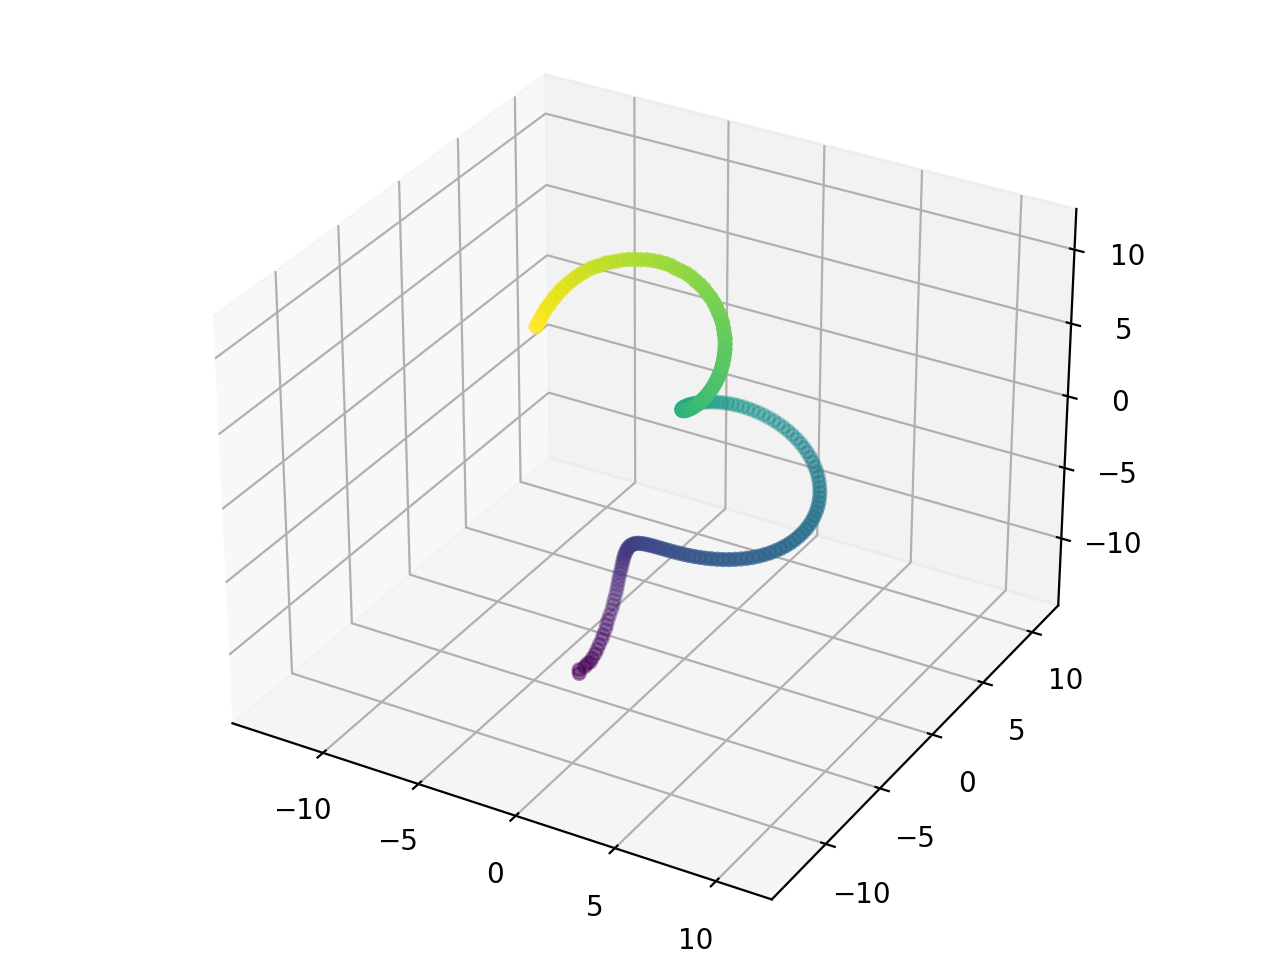
\includegraphics[trim=1cm 0cm 1cm 1cm, clip, width=0.45\textwidth]{Figures/mds_curve}
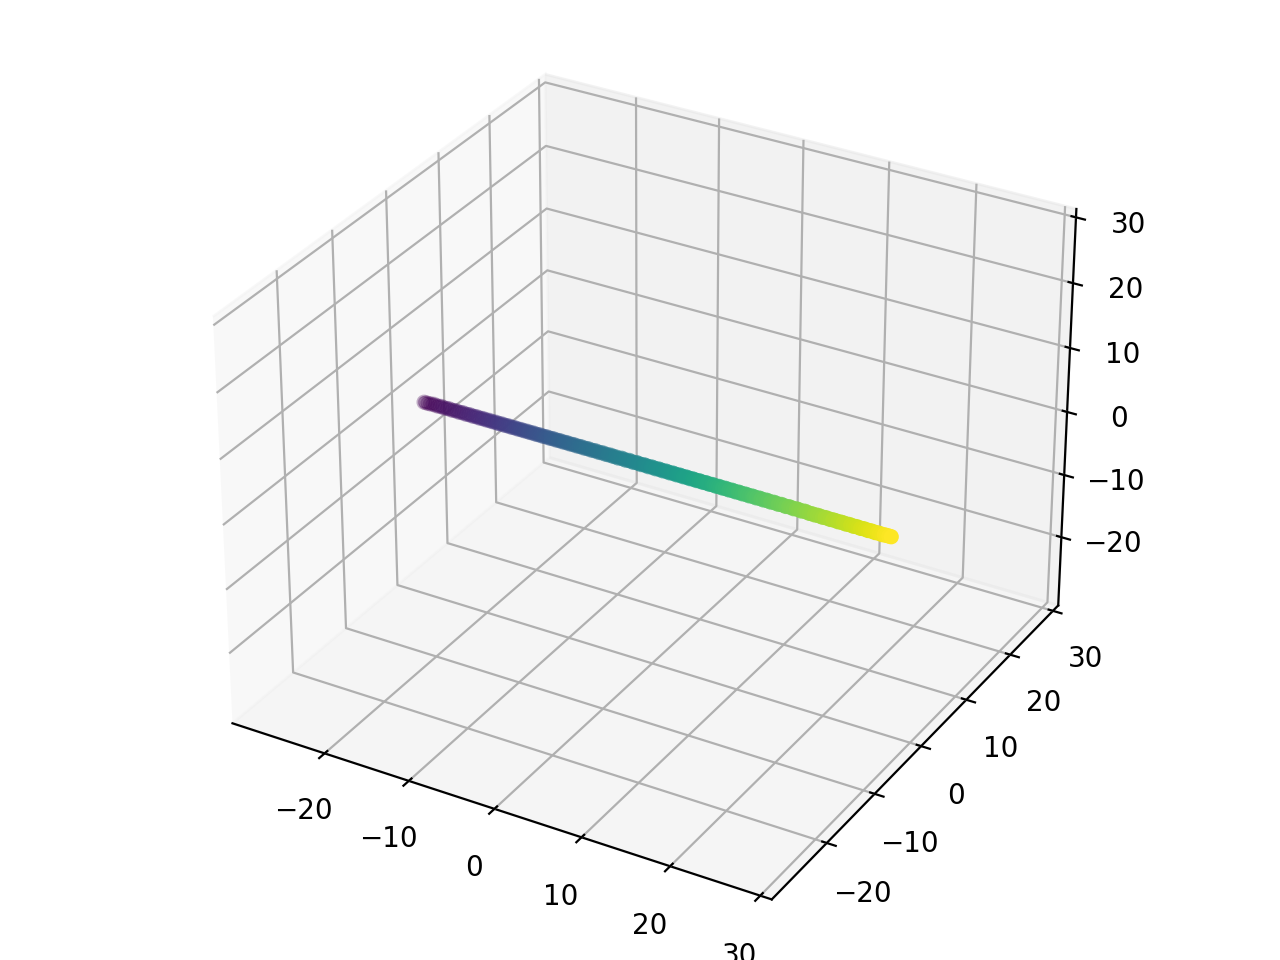
\includegraphics[trim=1cm 0cm 1cm 1cm, clip, width=0.45\textwidth]{Figures/isomap_curve}
\caption{\label{fig:isomap.curve} Left: Multidimensional scaling applied to a 3D curve embedded in a 10-dimensional space retrieves the Euclidean structure. Right: Isomap, in contrasts, identifies the one-dimensional nature of the data.} 
\end{figure}  


\subsection{Isomap}

Let us return to the example of people living on the spherical Earth. One can define the distance between two points on Earth either as the shortest length a person would have to travel (say, by plane) to go from one point to the other (that we can call the {\em intrinsic distance}), or simply the {\em chordal distance} in 3D space between the two points. The first one is obviously the most relevant to the spherical structure of the Earth, but the second one is  easier to compute given the locations of the points in space.  

For typical datasets, the geometric structure of the data (e.g., that it is supported by a sphere) is unknown, and the only information that is available is their chordal distance in an ambient space (which can be very large). An important remark, however is that, when the points are close to each other, the two distances can be expected to be similar, if we assume that the geometry of the set supporting the data is locally linear (e.g., that it is, like the sphere, a ``submanifold'' of the ambient space, with small neighborhoods of any data point well approximated, at first order, by points on a  tangent space).
Isomap uses this property, only trusting small distances in the matrix $D$, and infers large distances by adding the costs resulting from traveling from data points to nearby data points. 


%Let the training set  $T = (x_1, \ldots, x_N)$ be given in $\mR^d$ and
Fix an integer $c$.  
Given $D$, the $c$-nearest neighbor graph on $\CV = \{1, \ldots, N\}$ places an edge between $k$ and $l$ if and only if $d_{k,l}$ is among the $c$ smallest values in $\{d_{kl'}, l'\neq k\}$ neighbors or $x_l$ among the $c$ smallest values in  $\{d_{k'l}, k'\neq l\}$. We will write $k\sim_c l$ to indicate that there exists an edge between $k$ and $l$ in this graph.
 One then defines the geodesic distance on the graph as
\[
\pe{d_{kl}} * = \min\left\{ \sum_{j=1}^m d_{k_{j-1}k_{j}}: k_0, \ldots, k_m \in \{1, \ldots, N\}, k_0=k \sim_c k_1\sim_c \cdots \sim_c k_{m-1} \sim_c k_m=l, m\geq 0\right\}\,.
\]


This geodesic distance can be computed incrementally as follows. First define $d^{(1)}_{kl} = |x_k-x_l|$ if $k\sim_c l$ and   $ d^{(1)}_{kl} = +\infty$ otherwise (and also let $d^{(1)}_{kk}=0$). Then, given $d^{(n-1)}$, define
\[
d^{(n)}_{kl}  = \min\left\{d^{(n-1)}_{kl'} + d^{(1)}_{ll'}\: l'=1, \ldots, N\right\}
\]
until the entries stabilize, i.e., $d^{(n+1)} = d^{(n)}$, in which case one has $\pe d *=d^{(n)}$. The validity of the statement can be easily proved by checking that 
\[
d^{(n)}_{kl} = \min\left\{ \sum_{j=1}^n d^{(1)}_{k_{j-1}k_{j}}: k_0, \ldots, k_n \in \{1, \ldots, N\}, k_0=k, k_n=l\right\}\,,
\]
which can be done by induction, the details being left to the reader. It should also be clear that the procedure will stabilize after no more than $N$ steps.

Once the distance is computed, Isomap then  applies standard MDS, resulting in a straightened representation of the data like in \cref{fig:isomap.curve}. Another example is provided in \cref{fig:isomap.curve.closed}, where, this time, the input curve is closed and cannot therefore be represented as a one-dimensional structure. One can note, however, that, even in this case, Isomap still provides some simplification of the initial shape of the data.

\begin{figure}
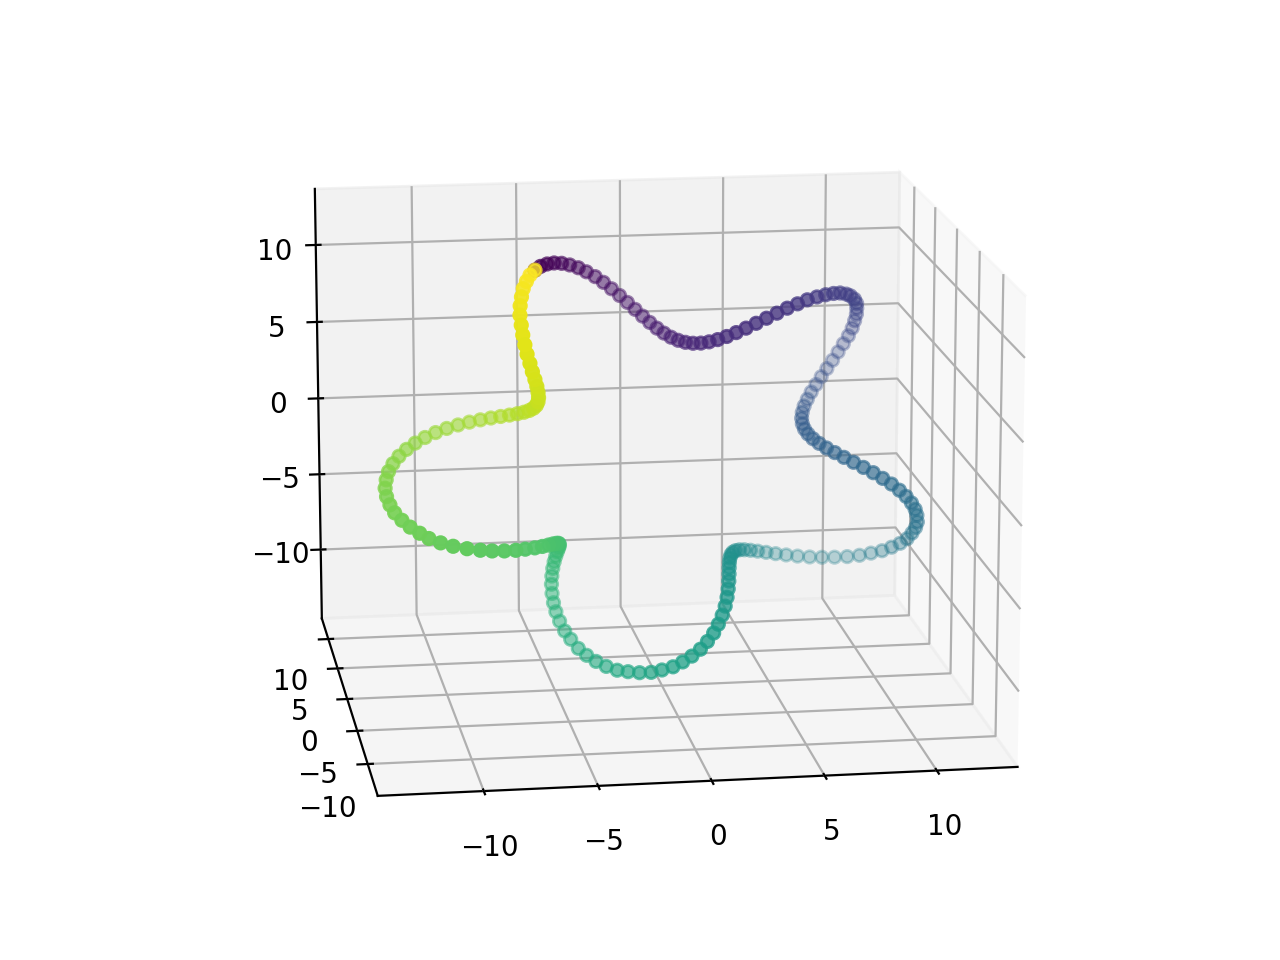
\includegraphics[trim=1cm 0cm 1cm 1cm, clip, width=0.45\textwidth]{Figures/mds_curve_closed}
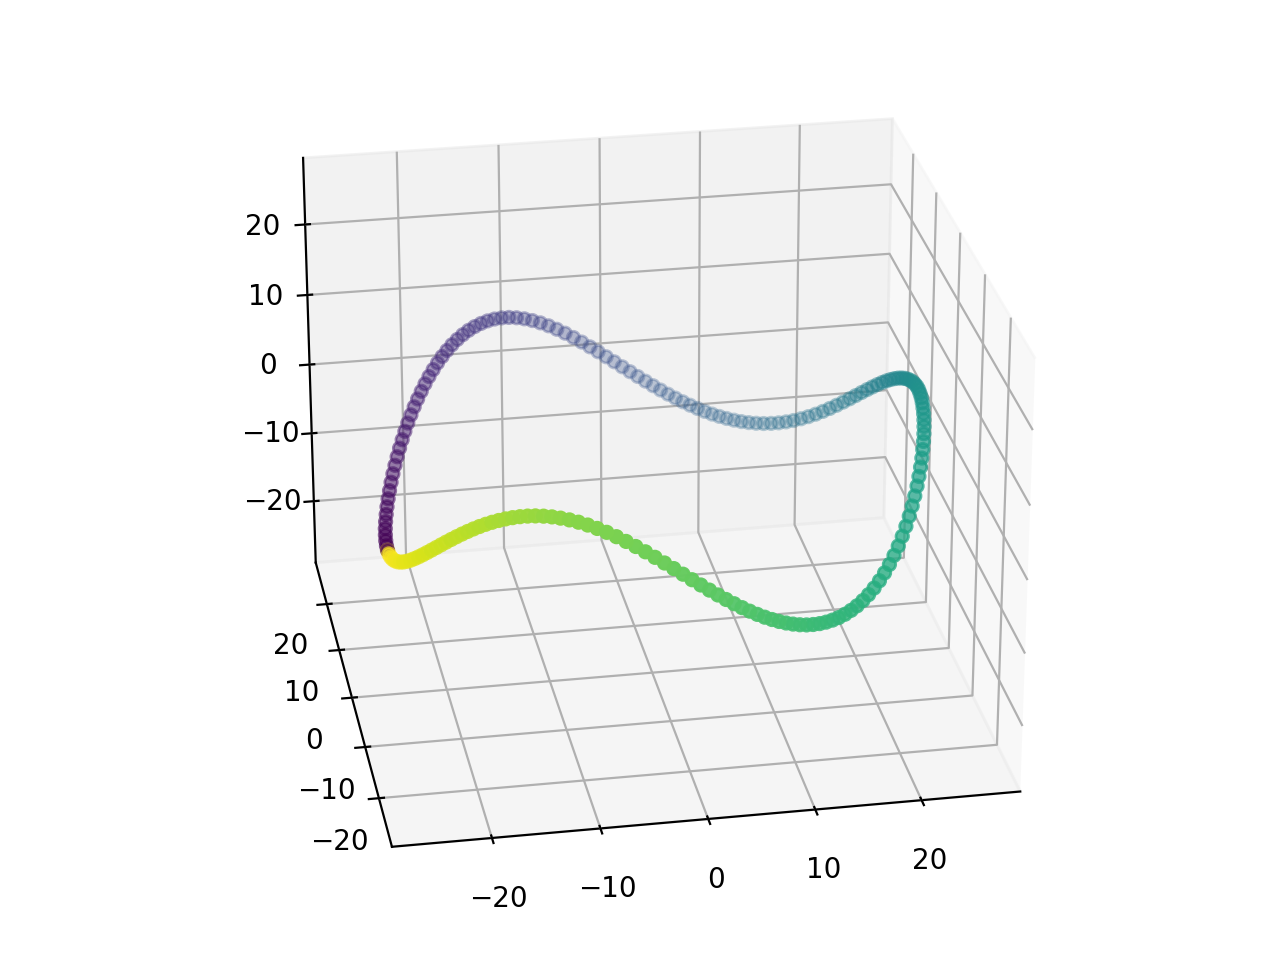
\includegraphics[trim=1cm 0cm 1cm 1cm, clip, width=0.45\textwidth]{Figures/isomap_curve_closed}
\caption{\label{fig:isomap.curve.closed} Left: Multidimensional scaling applied to a 3D curve embedded in a 10-dimensional space retrieves the Euclidean structure. Right: Isomap, in contrasts, identifies the one-dimensional nature of the data.} 
\end{figure}  



\subsection{Local Linear Embedding}
\label{sec:lle}
Local linear embedding (LLE) exploits in a different way the fact that manifolds are locally well approximated by linear spaces. Like Isomap, it starts also with building a $c$-nearest-neighbor graph on $\{1, \ldots, k\}$. Assume, for the sake of the discussion, that the distance matrix is computed for possibly unobserved data $T = (x_1, \ldots, x_N)$. 
Letting $\CN_k$ denote the indices of the nearest neighbors of $k$ (excluding $k$ itself), the basic assumption is that $x_k$ should approximately lie in the affine space generated by $x_l, l\in \CN_k$. Expressed in barycentric coordinates, this space is defined by
\[
\CT_k = \defset{ \sum_{l\in\CN_k} \pe \rho l x_l : \rho\in \mR^{\CN_k}, \sum_{l\in \CN_k} \pe \rho l = 1},
\]
and $\CT_k$ can be interpreted as an approximation of the tangent space at $x_k$ to the data manifold. Optimal coefficients $(\pe \rho_{k} l, k=1, \ldots, N, l\in\CN_k)$ providing the representation of $x_k$ in that space can be estimated by minimizing, for all $k$
\[
\left |x_k - \sum_{\l\in\CN_k}\pe {\rho_{k}} l x_l \right|^2
\]  
subject to $\sum_{l\in \CN_k} \pe {\rho_{k}} l = 1$. This is a simple least-square program. Let $c_k = |\CN_k|$ ($c_k=c$ in the absence of ties).
Order the elements of $\CN_k$ to represent $\pe{\rho_{k}} l, l\in\CN_k$ as a vector denoted $\bfrho_k\in \mR^{c_k}$. Similarly, let $S_k$ be the Gram matrix associated with $x_l, l\in\CN_k$ formed with all inner products $x_{l'}^T x_l$, $l,l'=1, \ldots, N$ and let $\bfr_k$ be the vector composed with products $x_k^Tx_l, l\in\CN_k$. Assume that $S_k$ is invertible, which is generally true if $c < d$, unless the neighbors are exactly linearly aligned. Then, the optimal $\bfrho_k$ and the Lagrange multiplier $\la$ for the constraint are given by
\begin{equation}
\label{eq:lle.1}
\begin{pmatrix} \bfrho_k\\ \la\end{pmatrix} = 
\begin{pmatrix} S_k & \dsone_{c_k}\\
\dsone_{c_k}^T & 0
\end{pmatrix}^{-1}
\begin{pmatrix} \bfr_k\\ 1\end{pmatrix}.
\end{equation}
If  $S_k$ is not invertible, the problem is under-constrained and one of its solutions can be obtained by  replacing the inverse above by a pseudo-inverse.

The low-dimensional representation of the data, still denoted $(y_1, \ldots, y_N)$ with $y_k\in\mR^p$ is then estimated so that the relative position of $y_k$ to its neighbors is the same as that of $x_k$, i.e., so that
\[
y_k \simeq \sum_{l\in\CN_k} \pe {\rho_{k}} l y_l.
\]
These vectors are estimated by minimizing
\[
F(y) = \sum_{k=1}^N \left| y_k - \sum_{l\in \CN_k} \pe{\rho_{k}}l y_l\right|^2.
\]
Obviously, some additional constraints are needed to avoid the trivial solution $y_k = 0$ for all $k$. Also, replacing all $y_k$'s by $y_k' = Ry_k + b$ where $R$ is an orthogonal transformation in $\mR^p$ and $b$ is a translation does not change the value of $F$, so there is no loss of generality in assuming that $\sum_{k=1}^N y_k = 0$ and that $\sum_{k=1}^N y_ky_k^T = D_0$, a diagonal matrix. However, if one lets $y'_k = Dy_k$ where $D$ is diagonal, then
\[
F(y) = \sum_{i=1}^p D_{ii}^2 \sum_{k=1}^N \left( \pe{y_k}i - \sum_{l\in \CN_k} \pe{\rho_{k}}l \pe{y_l}i\right)^2.
\]
This shows that one should not allow the diagonal coefficients of $D_0$ to be chosen freely, since otherwise the optimal solution would require to take this coefficient to $0$. So $D_0$ should be a fixed matrix, and by symmetry, it is natural to take $D_0 = \Id[p]$. (Any other solution---for a different $D_0$---can then be obtained by rescaling independently the coordinates of $y_1, \ldots, y_N$.)

Extend $\pe{\rho_{k}}l$ to an $N$-dimensional vector by taking $\pe{\rho_{k}}k = -1$ and $\pe{\rho_{k}}l=0$ if $l\neq k$ and $l\not \in \CN_k$. We can write 
\[
F(y) = \sum_{k=1}^N \left |\sum_{l=1}^N \pe{\rho_{k}}l y_l \right|^2.
\]
Expanding the square, this is
\[
F(y) = \sum_{l,l'=1}^N w_{ll'} y_l^Ty_{l'}
\]
with $w_{ll'} = \sum_{k=1}^N \pe{\rho_{k}}l \pe{\rho_{k}}{l'}$. Introducing the matrix $\CW$ with entries $w_{kl}$ and the $N\times p$ matrix $\CY = \begin{pmatrix}
y_1^T \\\vdots \\y_N^T
\end{pmatrix}
$, we have the simple expression
\[
F(y) =  \trace(\CY^T \CW \CY)\,.
\]
Note that the constraints are $\CY^T\CY = \Id[p]$ and $\CY^T \dsone_N = 0$. Without this last constraint, we know that an optimal solution is provided by $\CY = [e_1, \ldots, e_p]$ where $e_1,\ldots, e_p$ provide an orthonormal family of eigenvectors associated to the $p$ smallest eigenvalues of $\CW$ (this is a consequence of \cref{cor:pca.base}).  To handle the additional constraint, it suffices to note that $\CW \dsone_N = 0$, so that $\dsone_N$ is a zero eigenvector. Given this, it suffices to compute   $p+1$ eigenvectors associated to smallest eigenvalues of $\CW$, $e_1,\ldots, e_{p+1}$, with the condition that $e_1 = \pm \dsone_N/\sqrt N$ (which is automatically satisfied unless 0 is a multiple eigenvalue of $\CW$) and let 
\[
\CY = [e_2, \ldots, e_{p+1}].
\]
Note that $e_2, \ldots, e_{p+1}$ are also the $p$ smallest eigenvectors of $\CW + \la \dsone\dsone^T$ for any large enough $\la$, e.g., $\la > \trace(\CW)/N$.

LLE is summarized in the following algorithm.
\begin{algorithm}[Local linear embedding]
\label{alg:lle}
The input of the algorithm is 
\begin{enumerate}[label= (\roman*),wide=1cm]
\item Either a training set $T = (x_1, \ldots, x_N)$, or its Gram matrix $S$ containing all inner products $x_k^T x_l$ (or more generally inner products in feature space), or a dissimilarity matrix $D = (d_{kl})$. 
\item An integer $c$ for the graph construction.
\item An integer $p$ for the target dimension.
\end{enumerate}
\begin{enumerate}
\item If not provided in input, compute the Gram matrix $S$ and distance matrix $D$ (using \cref{eq:s.to.d} and \cref{eq:dissim.sim}).
\item Build the $c$-nearest-neighbor graph associated with the distances. Let $\CN_k$ be the set of neighbors of $k$, with $c_k = |\CN_k|$.
\item For $k=1, \ldots, N$, let $S_k$ be the sub-matrix of $S$ matrix associated with $x_l, l\in \CN_k$ and compute coefficients $\pe {\rho_{k}}l, l\in \CN_k$ stacked in a vector $\bfrho_k\in \mR^{c_k}$ by solving \cref{eq:lle.1}.
\item  Form the matrix $\CW$ with entries  $w_{ll'} = \sum_{k=1}^N \pe{\rho_{k}}l \pe{\rho_{k}}{l'}$ with $\rho$ extended so that $\pe{\rho_{k}}k = -1$ and $\pe{\rho_{k}}l=0$ if $l\neq k$ and $l\not \in \CN_k$.
\item Compute the first $p+1$ eigenvectors, $e_1, \ldots, e_{p+1}$, of $\CW$ (associated with smallest eigenvalues) arranging for $e_1$ to be proportional to $\dsone_N$.
\item Set $\pe{y_k}i = \pe{e_{i+1}}k$ for $i=1, \ldots, p$ and $k=1, \ldots, N$.
\end{enumerate}
\end{algorithm}
The results of LLE applied to the datasets described in \cref{fig:isomap.curve} and \cref{fig:isomap.curve.closed} are provided in \cref{fig:lle.curve}.
\begin{figure}
\centering
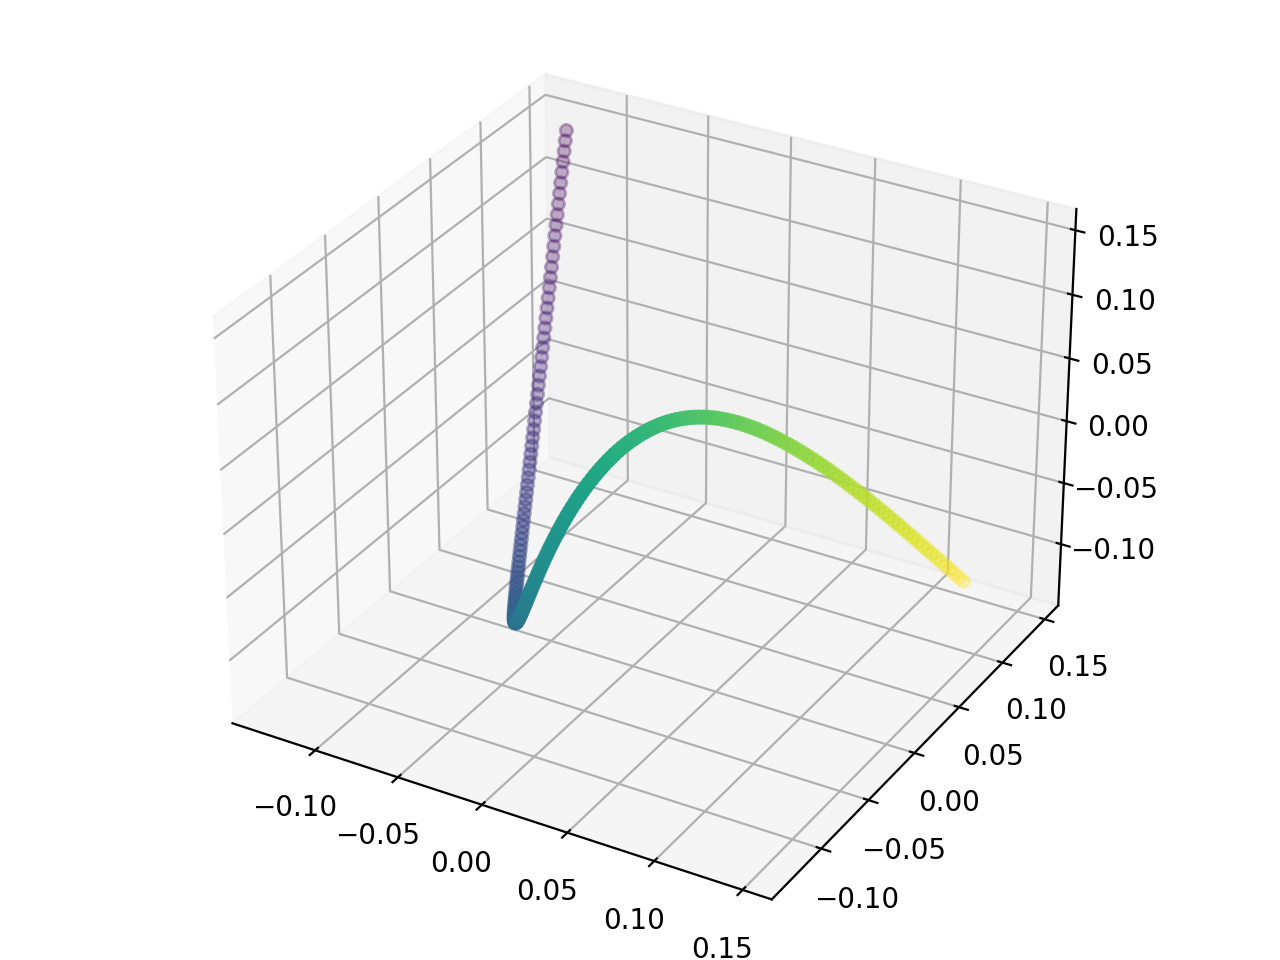
\includegraphics[trim=1cm 0cm 1cm 1cm, clip, width=0.45\textwidth]{Figures/lle_curve}
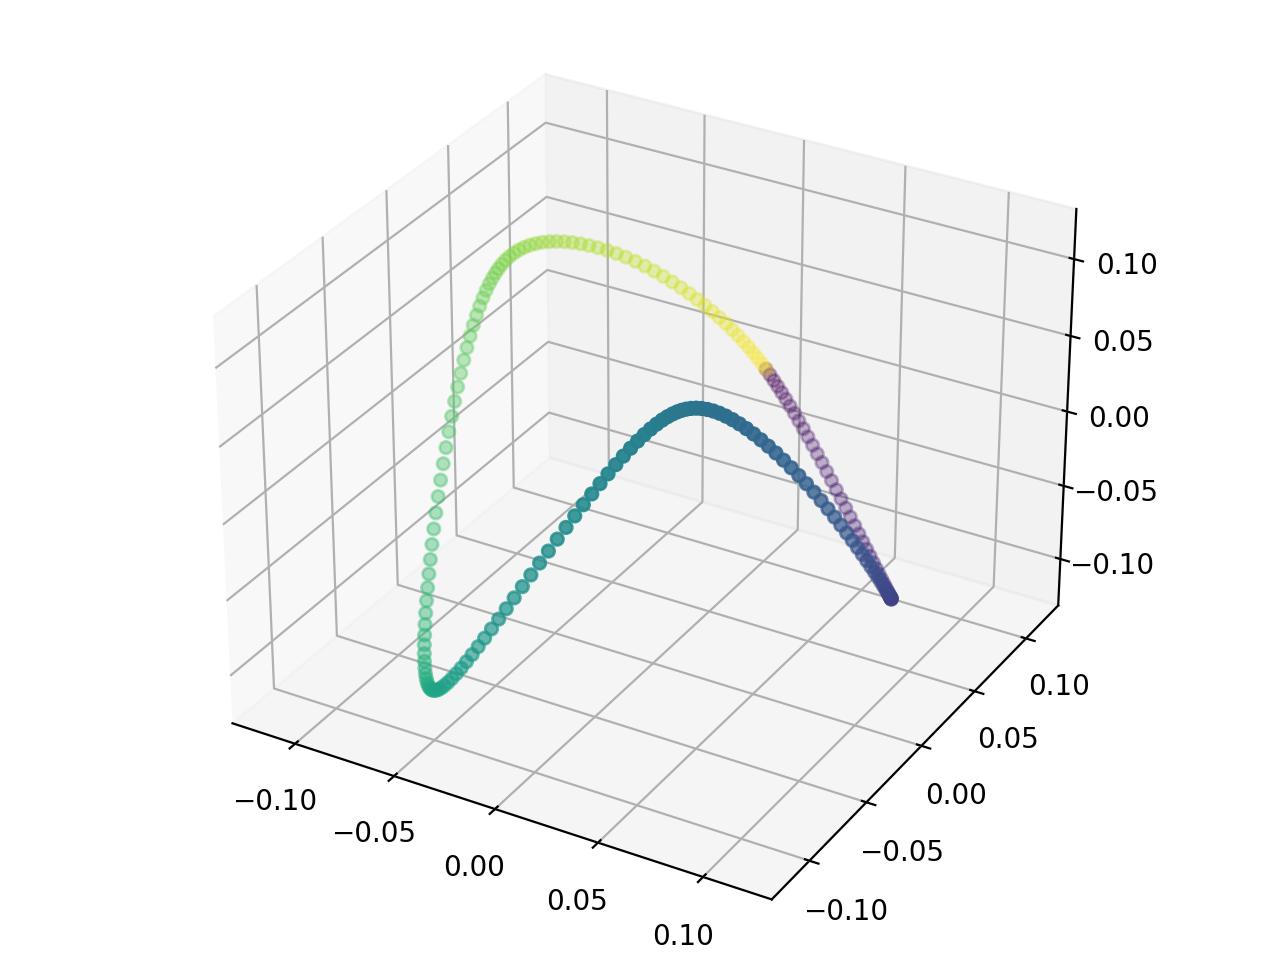
\includegraphics[trim=1cm 0cm 1cm 1cm, clip, width=0.45\textwidth]{Figures/lle_curve_closed}
\caption{\label{fig:lle.curve} Local linear embedding with target dimension $3$ applied to the data in \cref{fig:isomap.curve} and \cref{fig:isomap.curve.closed}.} 
\end{figure}

\begin{remark}
We note that, for both Isomap and LLE, the $c$-nearest-neighbors graph can be replaced by the graph formed with edges between all pairs of points that are at distance less than $\ep$ from each other, for a chosen $\ep>0$, with no change in the algorithms.

These parameters ($c$ or $\ep$) must be chosen carefully and may have an important impact on the output of the algorithm. Choosing them too small would not allow for a correct estimation of distances in Isomap (with possibly some of them being infinite if the graph has more than one connected component), or of the linear approximations in LLE. However, choosing them too large
may break the basic hypothesis that the data is locally Euclidean or linear that form the basic principles of these algorithms.
\end{remark}


\subsection{Graph Embedding}

Both Isomap and LLE  are based on the construction of a nearest-neighbor graph based on dissimilarity data and the conservation of some of its geometric features when deriving a small-dimensional representation. For LLE, a weight matrix $\CW$ was first estimated based on optimal linear approximations of $x_k$ by its neighbors, and the representation was computed by estimating the eigenvectors associated with the smallest eigenvalues of $\CW$ (excluding the eigenvector proportional to $\dsone$). However, both methods were motivated by the intuition that the dataset was supported by a continuous small-dimensional manifold.
We now discuss methods that are solely motivated by the discrete geometry of a graph, for which we use tools that are similar to our discussion of graph clustering in \cref{sec:graph.cluster}. 

Adapting the notation in that section to the present one, we start with a graph with $N$ vertices and weights $\be_{kl}$ between these vertices (such that $\be_{ll}=0$) and we form the Laplacian operator defined by, for any vector $u\in \mR^N$:
\[
\frac12 \|u\|_{H^1} = \frac12 \sum_{l,l'=1}^N \be_{ll'} (\pe u l - \pe u{l'})^2 = u^TLu, 
\]
so that $L$ is identified as the matrix with coefficients $\ell_{ll'} = - \be_{ll'}$ for $l\neq l'$ and $\ell_{ll} = \sum_{l'=1}^N \be_{ll'}$. The matrix $\CW$ that was obtained for LLE coincides with this graph Laplacian if one lets $\be_{ll'} = - w_{ll'}$ for $l\neq l'$, since we have $\sum_{l'=1}^N w_{ll'} = 0$. The usual requirement that weights are non-negative is no real loss of generality, because in LLE (and in the Graph embedding method above), one is only interested in eigenvectors of $\CW$ (or $L$ below) that are perpendicular to $\dsone$, and those remain the same if one replaces $\CW$ by
\[
\CW - a \dsone_N\dsone_N^T + Na \Id[N]
\]
which has negative off-diagonal coefficients $\tilde w_{ll'} = w_{ll'} - a$ for large enough $a$.
   

In graph (or Laplacian) embedding, the starting point is a weighted graph on $\{1, \ldots, N\}$ with edge weights $\be_{ll'}$ interpreted as similarities between vertexes. These weights may or may not be deduced from measures of dissimilarity $(d_{ll'}, k,l=1, \ldots, N)$ which themselves may or may not be computed as distances between training data $x_1, \ldots, x_N$. If one starts with dissimilarities, it is typical to use simple transformations to compute edge weights, and one the most commonly used is
\[
\be_{ll'} = \exp(-d_{ll'}^2/2\tau^2)
\]
for some constant $\tau$. These weights are usually truncated, replacing small values by zeros (or the computation is restricted to nearest neighbors), to ensure that the resulting graph is sparse, which speeds up the computation of eigenvectors for large datasets. 

Given a target dimension $p$, the graph is then represented as a collection of points $y_1, \ldots, y_N\in \mR^p$, where $y_k$ is associated to vertex $k$. For this purpose, one needs to compute the first $p+1$ eigenvectors, $e_1, \ldots, e_{p+1}$, of the graph Laplacian, with the requirement that $e_1 = \pm \dsone_N/\sqrt{N}$. (This is always possible and  can be achieved numerically by computing eigenvectors of $L + c\dsone\dsone^T$ for large enough $c$.) The graph representation is then given by  $\pe {y_k}|i = \pe{e_{i+1}}k$ for $i=1, \ldots, p$ and $k=1, \ldots, N$. Note that these are exactly the same operations as those described in steps 4 and 5 of the LLE algorithm. 

One way to interpret this construction is that $e_2, \ldots, e_{p+1}$ (the coordinate functions for the representation $y_1, \ldots, y_N$) minimize
\[
\sum_{j=1}^p \|e_i\|^2_{H_1}
\]
subject to $e_2, \ldots, e_{p+1}$ being perpendicular to each other and perpendicular to the constant functions (these constraints being justified for the same reasons as those discussed for LLE). Small $H^1$ semi-norms being associated with smoothness on the graph, we see that we are looking for the smoothest zero-mean representation of the data.

Based on our discussion of LLE, we can make an alternative interpretation by introducing a symmetric square root $R$ of the Laplacian matrix $L$ or any matrix such that $RR^T = L$. Writing $R = [\bfrho_1, \ldots, \bfrho_N]$, one has
\[
L = \sum_{k=1}^N \bfrho_k \bfrho_k^T
\]
and $\sum_{k=1}^N  \bfrho_k = 0$. With this notation, we can interpret Laplacian embedding as the minimization of
\[
\sum_{k=1}^N \left| \sum_{l=1}^N \pe{\rho_{k}}l y_l\right|^2
\]
(subject to previous orthogonality constraints). In other terms, $y_1, \ldots, y_N$ are determined so that the linear relationships
\[
\rho_{kk} y_k = -\sum_{l\neq k} \pe{\rho_{k}}l y_l
\]
are satisfied, which is similar to the LLE condition, without the requirement that $\rho_{k}(k) = 1$. 

An alternate requirement that could have been made for LLE is that $\sum_{l=1}^N (\pe{\rho_{k}}l)^2 = 1$ for all $k$. Instead of having to solve a linear system in step 2 of \cref{alg:lle}, one would then compute an eigenvector with smallest eigenvalue of $S_k$. For graph embedding, this constraint can be enforced by modifying the Laplacian matrix, since $\sum_{l=1}^N (\pe{\rho_{k}}l)^2$ is just the $(k,k)$ coefficient of $RR^T$. Given this, let $D$ be the diagonal matrix formed by the diagonal elements of $L$, and define the so-called ``symmetric Laplacian'' $\tilde L = D^{-1/2} L D^{-1/2}$. One obtain an alternative, and popular, graph embedding method by replacing $e_1, \ldots, e_{p+1}$ above by the first $p$ eigenvectors of $\tilde L$.

\bigskip

Another interpretation of this representation can be based on the random walk associated with the graph structure. Consider the random process $t \mapsto \bfq(t)$ defined as follows. The initial position, $\bfq(0)$ is selected according to some arbitrary distribution, say $\pi_0$. Conditional to $\bfq(t) = k$, the next position is determined by setting random waiting times $\tau_{kl}$, each distributed as an exponential distribution with rate $\be_{kl}$ (or expectation $1/\be_{kl}$), and the process moves to the position $l$ for which $\tau_{kl}$ is smallest after waiting for that time. Let  $P(t)$ be the matrix with coefficients $P(t, k, l) = P(\bfq(t+s) = l\mid \bfq(s) = k)$. Then, one has
\[
P(t) = e^{-t L}
\]
where the right-hand side is the matrix exponential. If $\la_1 = 0 \leq \lambda_2 \leq\cdots \leq \la_N$ are the eigenvalues of $L$ with corresponding eigenvectors $e_1, \ldots, e_N$, then
\[
P(t) = \sum_{i=1}^N e^{-t\la_i} e_ie_i^T
\]
In particular, restricting the first eigenvectors of $L$ provides an approximation of this stochastic process, i.e., 
\[
P(t) \simeq \frac{\dsone\dsone^T}N + \sum_{i=1}^p e^{-t\la_{i+1}} y(i)y(i)^T.
\] 

We could also have considered the discrete-time version of the walk, for which, considering integer times $t\in \mN$, 
\[
P(\bfq(t+1) = l \mid \bfq(t) = k) =\left\{
\begin{aligned}
 \frac{\be_{kl}}{\sum_{l'=1, l'\neq k}^N \be_{kl'}} \text{ if } l\neq k\\
 0 \text{ if } l=k
 \end{aligned}
 \right.
\]
Introducing the matrix $B$ of similarities $\be_{kl}$ (with zero on the diagonal) and the diagonal matrix $D$ with coefficients 
$d_{kk} = \sum_{l =1, l\neq k}^N \be_{kl}$, the r.h.s. of the previous equation is the $k,l$ entry of the matrix $\tilde P = D^{-1} B$. Then, for any integer $s$, $P(\bfq(t+s) = l \mid \bfq(t) = k)$ is the $k,l$ entry if $\tilde P^s = D^{-1/2} (D^{-1/2} B D^{-1/2})^s D^{1/2}$.

The Laplacian matrix $L$ is given by $L = D-B$. The normalized Laplacian is 
\[
\bar L = D^{-1/2} L D^{-1/2} = \Id[N] - D^{-1/2} B D^{-1/2}
\]
so that
\[
\tilde P^s = D^{-1/2} (\Id[N] - \bar L)^s D^{1/2}.
\]
If one introduces the eigenvectors $\bar e_1, \ldots, \bar e_N$ of the normalized Laplacian, still associated with non-decreasing eigenvalues $\bar\la_1=0, \ldots, \bar\la_N$, and arranges without loss of generality that $\bar e_1 \propto D^{1/2} \dsone_N$, then 
\[
\tilde P^s = D^{-1/2} \left(\sum_{i=1}^N (1 - \bar \la_i)^s \bar e_i\bar e_i^T\right) D^{1/2}.
\]
This shows that, for $s$ large enough, the transitions of this Markov chain are well approximated by its first terms, suggesting using the alternative representation based on the normalized Laplacian:
\[
\bar y_k(i) = \bar e_{i+1}(k).
\]
Both representations (using normalized or un-normalized Laplacians) are commonly used in practice.

 

\subsection{Stochastic neighbor embedding}

\subsubsection{General algorithm}
Stochastic neighbor embedding (SNE, \citet{hinton2002stochastic}), and its variant (t-SNE, \citet{maaten2008visualizing}) have become a popular tool for the visualization of high-dimensional data based on dissimilarity matrices. One of the key contributions of this algorithm is to introduce a local data rescaling step, that allows for visualization of more homogeneous point clouds. 

Assume that dissimilarities $D = (d_{kl}, k,l=1, \ldots, N)$ are observed. The basic principle in SNE is to deduce from the dissimilarities a family of $N$ probability distributions on $\{1, \ldots, N\}$, that we will denote $\pi_k$, $k=1, \ldots, N$, with the property that $\pi_k(k) = 0$. The computation of these probabilities include the local normalization step, and we will return to this later. Given the $\pi_k$'s, one then estimate low-dimensional representations $\bfy = (y_1, \ldots, y_N)$ such that $\pi_k \simeq \psi_k$ where $\psi_k$ is given by
\[
\psi_k(l;\bfy) = \frac{\exp\big(-\beta\big(|y_k-y_l|^2\big)\big)}{\sum_{l'=1, l'\neq k}^N \exp\big(-\beta\big(|y_k-y_{l'}|^2\big)\big)} \bfone_{l\neq k}.
\] 
Here, $\beta: [0, +\infty) \to [0, +\infty)$ is an increasing differentiable function that tends to $+\infty$ at infinity. The  derivative is denoted $\prt\be$. The original version of SNE \citep{hinton2002stochastic} uses $\beta(t) = t$ and t-SNE \citep{maaten2008visualizing} takes $\beta(t) = \log(1+t)$.  

%One can interpret the probabilities $\pi_k$ as defining a {\em random walk} on the set $\{1, \ldots, N\}$, where  the probability of moving from $k$ to $l$ is given by $\pi_k(l)$. The goal of SNE is to make the chain associated with $\psi$ as close as possible to that provided by $\pi$.

The determination of the representation can then be performed by minimizing a measure of discrepancy between the probabilities $\pi_k$ and $\psi_k$. In \citet{hinton2002stochastic}, it is suggested to minimize the sum of Kullback-Liebler divergences, namely
\[
\sum_{k=1}^N \KL(\pi_k\|\psi_k(\cdot;\bfy)) 
\]
or, equivalently, to maximize
\begin{align*}
F(\bfy) &= \sum_{k,l=1}^N \pi_k(l) \log \psi_k(l ; \bfy) \\
&= - \sum_{k,l=1}^N \be(|y_k-y_l|^2) \pi_k(l) + \sum_{k=1}^N \log \left(\sum_{l=1, l\neq k}^N \exp(-\be(|y_k-y_l|^2))\right)
\end{align*}
The gradient of this function can be computed by evaluating the derivative at $\ep=0$ of $f: \ep \mapsto F( \bfy+\ep \bfh)$. This computation gives
\begin{align*}
f'(0) =& -2 \sum_{k,l=1}^N \prt\be(|y_k-y_l|^2) (y_k-y_l)^T(h_k-h_l) \pi_k(l) \\
&+ 2\sum_{k=1}^N \sum_{l=1}^N \prt \be(|y_k-y_l|^2) (y_k-y_l)^T(h_k-h_l)\psi_k(l;\bfy)\\
 =& - 2 \sum_{k=1}^N h^T_k \sum_{l=1}^N \prt\be(|y_k-y_l|^2)(y_k - y_l) (\pi_k(l) + \pi_l(k) - \psi_k(l;\bfy) - \psi_l(k;\bfy))
\end{align*}
This shows that
\[
\prt_{y_k} F(\bfy) = -2  \sum_{l=1}^N \be(|y_k-y_l|^2)(y_k - y_l) (\pi_k(l) + \pi_l(k) - \psi_k(l;\bfy) - \psi_l(k;\bfy)).
\]

This is a rather simple expression that can be used with any first-order optimization algorithm to maximize $F$. The algorithm in
\citet{hinton2002stochastic} uses gradient ascent with momentum, namely iterating 
\[
\bfy^{(n+1)} = \bfy^{(n)} + \gamma \nabla F(\bfy^{(n)}) + \alpha^{(n)} (y^{(n)} - y^{(n-1)})
\]
Choosing $\alpha^{(n)} = 0$ provides standard gradient ascent with fixed gain $\gamma$ (of course,  other optimization methods may be used). The momentum can be interpreted, in a loose sense, as a ``friction term''.

\bigskip
A variant of the algorithm replaces the node-dependent probabilities $\pi_k$ by a single, symmetric, joint distribution $\bar\pi$ on $\{1, \ldots, N\}^2$, $(k,l) \mapsto \bar\pi(k,l)$, satisfying $\bar\pi(k,k) = 0$ and $\bar\pi(k,l) = \bar\pi(l,k)$.  The target distribution $\bar\psi$ then becomes 
\[
\bar\psi(k,l;\bfy) =    \frac{\exp(-\be(|y_k-y_l|^2))}{\sum_{k'\neq l'=1}^N \exp(-\be(|y_{k'} - y_{l'}|^2))}.
\]
With such a choice, the objective function has a simpler form,  namely minimizing $\KL(\bar\pi\|\bar\psi(\cdot, y))$ or maximizing the expected likelihood
\[
\bar F(\bfy) = \sum_{k,l=1}^N \bar \pi(k,l) \log\bar \psi(k,l; y) = -\sum_{k,l=1}^N \be(|y_k-y_l|^2) \bar\pi(k,l) + \log \left(\sum_{k\neq l=1}^N \exp(-\be(|y_k-y_l|^2))\right).
\] 
The gradient of this symmetric version of $F$ can be computed similarly to the previous one and is given by
\[
\prt_{y_k} \bar F(\bfy) = -4  \sum_{l=1}^N \prt\be(|y_k-y_l|^2) (y_k - y_l) (\bar\pi_(k, l) - \bar\psi(k, l;\bfy)).
\]

\subsubsection{Setting initial probabilities}

The probabilities $\pi_k(l)$ or $\bar\pi(k,l)$ are deduced from the dissimilarities as
\[
\pi_k(l) = \frac{e^{-d_{kl}^2/2\sigma^2_k}}{\sum_{l'=1, l'\neq k}^Ne^{-d_{kl'}^2/2\sigma^2_k}}
\]
for $l\neq k$ and 
\[
\bar\pi(k,l) = \frac{\pi_k(l) + \pi_l(k)}{2n}.
\]

The coefficients $\sigma^2_k$, $k=1, \ldots, N$ operate the local normalization, justifying, in particular, the parameter-free expression chosen for $\psi$ and $\bar\psi$. These coefficients are estimated
so as to adjust the entropies of all $\pi_k$ to a fixed value, which is a parameter of the algorithm. Note that, letting $t = 1/2\sigma_k^2$
and $H(\pi_k) = -\sum_{l=1}^N \pi_k(l) \log\pi_k(l)$, 
\begin{align*}
\prt_t H(\pi_k) &= - \sum_{l=1}^N \prt_t \pi_k(l) \log\pi_k(l) - \sum_{l=1}^N \prt_t \pi_k(l) \\
&= - \sum_{l=1}^N \prt_t \pi_k(l) \log\pi_k(l)
\end{align*}
Now
\[
\prt_t \log \pi_k(l) = - d_{kl}^2 + \bar d^2_k 
\]
with $\bar d_k^2 = \sum_{l'=1}^N d_{kl'}^2 \pi_k(l')$.
Writing $\prt_t \pi_k(l) = \pi_k(l) \prt_t\log\pi_k(l)$, we have
\[
\prt_t H(\pi_k) = \sum_{l=1}^N (d_{kl} \log\pi_k(l)) \pi_k(l)  - \bar d_k \sum_{l=1}^N \pi_k(l) \log\pi_k(l).
\]
Using Schwartz inequality, we see that $\prt_t H(\pi_k) \leq 0$ so that $H(\pi_k)$ is decreasing as a function of $t$, i.e., increasing as a function of $\sigma^2_k$. When $\sigma_k^2\to 0$, $\pi_k$ converges to the uniform distribution on the set of nearest neighbors of $k$ (the indexes $l\neq k$ such that $d_{kl}^2$ is minimal) and, letting $\nu_k$ denote their number, which is typically equal to 1, $H(\pi_k)$ converges to $\log\nu_k$. When $\sigma^2_k$ tends to infinity, $\pi_k$ converges to the uniform distribution over indexes $l\neq k$, whose entropy is $\log (N-1)$. This shows that $e^{H(\pi_k)}$, which is called the {\em perplexity} of $\pi_k$ can take any value between $\nu_k$ and $N-1$. The common target value of the perplexity can therefore be taken anywhere between $\max_k\nu_k$ and $N-1$. In \citet{maaten2008visualizing}, it is recommended to choose a value between 5 and 50.

\begin{remark}
The complexity of the computation of the gradient of the objective function (either $F$ or $\bar F$ ) scales like the square of the size of the training set, which may be prohibitive when $N$ is large. In \citet{van2014accelerating}, an accelerated procedure, that involves an approximation of the gradient is proposed. (This procedure is however limited to representations in dimensions 2 or 3.)
\end{remark}

\subsection{Uniform manifold approximation and projection (UMAP)}

UMAP is similar in spirit to t-SNE, with a few important differences that result in a simpler optimization problem and faster algorithms. Like Isomap, the approach is based on matching distances between the high-dimensional data and the low-dimensional representation. But while Isomap estimates a unique distance on the whole training set (the geodesic distance on the nearest-neighbor graph), UMAP estimates as many ``local distances'' as observations before ``patching'' them to form the final representation. 

The goal of transporting possibly non-homogeneous locally defined objects on initial data to a homogeneous low-dimensional visualization is what makes UMAP similar to t-SNE. The difference is that t-SNE transports local probability distributions, while UMAP transports metric spaces. More precisely, given distances $(d_{kl}, k,l=1, \ldots, N)$ and an integer $m$ provided as input, the algorithm builds, for each $k=1, \ldots, N$ a (pseudo-)metric $\delta_k$ on the associated data graph by letting
\[
\delta^{(k)}(k,l) = \delta^{(k)}(l,k) = \frac{1}{\sigma_k}\left(d_{kl} - \min_{l'\neq   k} d_{kl'}\right)
\]
if $l$ is among the $m$ nearest neighbors of $k$, where $m$ is a parameter of the algorithm, with all other distances being infinite. The normalization parameter $\sigma_k$ has a role similar to that of the same parameter in t-SNE in that it   tends to make the representation  homogeneous.  Here, it is computed such that
\[
\sum_l \exp(-\delta^{(k)}(l,l')) = \log_2 m\,.
\]
   
Each such metric provides a weighted graph structure on $\{1, \ldots, N\}$ by defining weights $w^{(k)}_{ll'} = \exp(-\delta^{(k)}(l,l'))$. 
In UMAP, these weights are interpreted in the framework of {\em fuzzy sets}, where a fuzzy set is defined by a pair $(A, \mu)$ where $A$ is a set and $\mu$ a function $\mu: A\to [0,1]$ \citep{zadeh1996fuzzy}. The function $\mu$ is called the membership function and $\mu(x)$ for $x\in A$ is the membership strength of $x$ to $A$.  Letting $\CV = \{1, \ldots, N\}$ and $\CE = \CV \times \CV$, one then interprets the weights as defining the membership strength of edges to the graph, i.e., one defines the ``fuzzy graph'' $\CG^{(k)} = (\CV, \CE, \mu^{(k)})$ where $\mu^{(k)}(l,l') = w^{(k)}_{ll'}$ is the membership strength of edge $(l,l')$ to  $\CG^{(k)}$.

This is, of course, just a reinterpretation of weighted graphs in terms of fuzzy sets, but it allows one to combine the collection $(\CG^{(k)}, k=1, \ldots, N)$ using simple fuzzy sets operations, namely, defining the combined (fuzzy) graph $\CG  = (\CV, \CE, \mu)$ with 
\[
(\CE, \mu) = \bigcup_{k=1}^N (\CE, \mu^{(k)})
\]
being the fuzzy union of the edge sets. There are, in fuzzy logic, multiple ways to define set unions \citep{gupta1991theory}, and the one selected for UMAP define $(A, \mu) \cup (A', \mu') = (A\cup A', \nu)$ with
$\nu(x) = \mu(x) + \mu'(x) - \mu(x)\mu'(x)$ ($\mu(x)$ and $\mu'(x)$ being defined as 0 is $x\not\in A$ or $x\not\in A'$ respectively).   In UMAP, each edge $\mu^{(k)}(l,l')$ is non-zero only is $k=l$ or $l'$ so that
\[
\mu(l,l') = w^{(l)}_{ll'} +  w^{(l')}_{ll'} -  w^{(l)}_{ll'} w^{(l')}_{ll'}.
\]  

This defines an input fuzzy graph structure on $\{1, \ldots, N\}$ that serves as target for an optimized similar structured associated with the representation $\bfy = (y_1, \ldots, y_N)$. This representation, since it is designed as a  homogeneous representation of the data, provides a unique fuzzy graph $\CH(\bfy) = (\CV, \CE, \nu(\cdot; \bfy))$ and the edge membership function is defined by $\nu(l,l';\bfy) = \phi_{a,b}(y_l, y_{l'})$ with
\[
\phi_{a,b}(y,y') = \frac{1}{1 + a |y-y'|^b}.
\]
The parameters $a$ and $b$ are adjusted so that $\phi_{a,b}$ provides a differentiable approximation of the function
\[
\psi_{\rho_0}(y,y') = \exp(- \max(0, |y-y'| - \rho_0))
\]
where $\rho_0$ is an input parameter of the algorithm. This function $\psi_{\rho_0}$ takes the same form as the membership function defined for local graphs $\CG^{(k)}$, and  its replacement by $\phi_{a,b}$ makes possible the use of gradient-based methods for the determination of the optimal $\bfy$ ($\psi_{\rho_0}$ is not differentiable everywhere).

The representation $\bfy$ is optimized by minimizing the ``fuzzy set cross-entropy''
\[
C(\mu\|\nu(\cdot, \bfy)) = \sum_{(k,l) \in \CE} \left(\mu(k,l) \log\frac{\mu(k,l)}{\nu(k,l|\bfy)} +(1- \mu(k,l)) \log\frac{1-\mu(k,l)}{1-\nu(k,l|\bfy)}\right)
\]
or, equivalently, maximizing (using, for short, $\phi = \phi_{a,b}$)
\begin{align*}
F(\bfy) &= \sum_{(k,l) \in \CE} \left(\mu(k,l) \log\nu(k,l|\bfy) +(1- \mu(k,l)) \log(1-\nu(k,l|\bfy))\right)\\
&= \sum_{(k,l) \in \CE} \left(\mu(k,l) \log\phi(y_k, y_{l}) +(1- \mu(k,l)) \log(1-\phi(y_k,y_{l}))\right)\\
\end{align*}

Note the important simplification compared to the similar function $F$ is t-SNE, in that the logarithm of a potentially large sum is avoided. We have
\begin{align*}
\prt_{y_k} F(\bfy) =& 2 \sum_{l=1}^N \mu(k,l) \prt_{y_k} \log\phi(y_k, y_{l}) + 2 \sum_{l=1}^N (1-\mu(k,l)) \prt_{y_k} \log(1-\phi(y_k, y_{l}))\\
=& 2 \sum_{l=1}^N \mu(k,l) \prt_{y_k} \log\frac{\phi(y_k, y_{l})}{1-\phi(y_k, y_{l})} + 2 \sum_{l=1}^N \prt_{y_k} \log(1-\phi(y_k, y_{l})).
\end{align*}
The optimization can be implemented using stochastic gradient ascent. Introduce random variables $\xi_{kl}$ and $\xi'_{kl}$ both taking value in $\{0,1\}$, all independent of each other and such that $P(\xi_{kl} = 1) = \mu_{kl}$ and $P(\xi'_{kl} = 1) = \epsilon$. Define
\[
H_k(\bfy, \xi, \xi') = 2 \sum_{l=1}^N \xi_{kl} \prt_{y_k} \log\frac{\phi(y_k, y_{l})}{1-\phi(y_k, y_{l})} + 2c_k  \sum_{l=1}^N\sum_{l'=1}^N \xi_{kl}\xi'_{kl'} \prt_{y_k} \log(1-\phi(y_k, y_{l'})).
\]
Then, if one takes $c_k = 1/(\epsilon\sum_{l} \mu(k,l))$ one has
\[
E(H_k(\bfy, \xi, \xi')) = \prt_{y_k} F(\bfy).
\]

 This corresponds to SGA iterations in which: 
\begin{enumerate}
\item Each edge $(k,l)$ is selected with probability $\mu(k,l)$ (which are zero for unless $k$ and $l$ are neighbors); 
\item If $(k,l)$ is selected, one selects an additional edges $(k,l')$ each with probability $\ep$.
\end{enumerate} 
Letting $l_1, \ldots, l_m$ be the number of edges selected,  $y_k$ is updated according to
\[
y_k \leftarrow y_k + 2\gamma \left(\prt_{y_k} \log\frac{\phi(y_k, y_{l})}{1-\phi(y_k, y_{l})} + c_k \sum_{j=1}^m 
\prt_{y_k} \log(1-\phi(y_k, y_{l'}))\right).
\]

\begin{remark}
If one prefers using probability rather than fuzzy set theory, the graphs $\CG^{(k)}$ may also be interpreted as random graphs in which edges are added independently from each other and each edge $(l,l')$  is drawn with probability $\mu^{(k)}(l,l')$. The combined graph $\CG$ is then the random graph in which $(l,l')$ is present if and only if it is in at least one of the $\CG^{(k)}$ and the objective function $C$ coincides with the KL divergence between this random graph and the random graph similarly defined for $\bfy$.

However, this fuzzy/random graph formulation of UMAP---which corresponds to current practical implementations---is only a special case of the theoretical construction made in \citet{mcinnes2020umap} which builds on the theory of (fuzzy) simplicial sets and their representation of metric spaces.  We refer the interested reader to this reference, which requires a mathematical background beyond the scope of these notes. 
\end{remark}

